\documentclass[aspectratio=169,10pt]{beamer}
\usetheme{default}
\usecolortheme{seahorse}
\usepackage{booktabs}
\usepackage{graphicx}
\setbeamertemplate{navigation symbols}{}
\setbeamertemplate{footline}[frame number]
\setbeamerfont{frametitle}{size=\large}
\newcommand{\qe}{Quantum ESPRESSO}

\title{\textbf{pypresso}}
\subtitle{Plane-wave DFT in Python and JAX, validated against \qe}
\date{2026-08-26}

\begin{document}

\begin{frame}\titlepage
\begin{center}\small
A ground-up reimplementation of \texttt{pw.x} --- \emph{not} a wrapper, not a binding.\\
Every number below is measured against \qe\ on the same input.
\end{center}
\end{frame}

% ---------------------------------------------------------------- 2
\begin{frame}{What it is, and why JAX}
\begin{columns}[T]
\column{0.52\textwidth}
\textbf{Two reasons, and both constrain the code:}
\begin{enumerate}
  \item \textbf{Autodifferentiation.} Forces, stress, phonons, dielectric
    response, Raman tensors come from \emph{differentiating the code}, not from
    separately hand-derived expressions.
  \item \textbf{GPU.} The same source runs on an accelerator unchanged.
\end{enumerate}
\vspace{4pt}
\textbf{The consequence that matters:}\\
QE's six hand-derived force terms, its stress terms, its \texttt{force\_hub} ---
these exist here as \emph{tests}, not as the implementation. One gradient
replaces them.
\column{0.44\textwidth}
\footnotesize
\begin{block}{Written down once, differentiated thereafter}
\begin{tabular}{ll}
\toprule
energy & written \\
$v_{xc}$ & \texttt{jax.grad} \\
force & \texttt{jax.grad} \\
stress & \texttt{jax.grad} \\
dyn.\ matrix & \texttt{jvp} of the force \\
$d\epsilon/d\tau$ (Raman) & \texttt{jvp} of $F_{ij}$ \\
\bottomrule
\end{tabular}
\end{block}
Third derivatives of $E_{xc}$ fall out of the same kernel, so a \textbf{GGA
Raman tensor} works where \texttt{ph.x} stops.
\end{columns}
\end{frame}

% ---------------------------------------------------------------- 3
\begin{frame}{Capabilities}
\scriptsize
\begin{columns}[T]
\column{0.5\textwidth}
\textbf{Ground state}
\begin{itemize}\itemsep1pt
  \item SCF, bands, DOS / PDOS, tetrahedra
  \item norm-conserving, \textbf{ultrasoft}, \textbf{PAW}
  \item LDA, PBE, revPBE, PBEsol; \textbf{meta-GGA} (TB09)
  \item metals: all smearings + tetrahedron occupations
  \item collinear spin, \textbf{noncollinear}, \textbf{spin-orbit}
  \item \textbf{DFT+U}, magnetic fields, constrained moments
  \item Grimme D2 dispersion
\end{itemize}
\textbf{Structure}
\begin{itemize}\itemsep1pt
  \item forces, stress, BFGS relax, \textbf{variable-cell} relax
\end{itemize}
\column{0.5\textwidth}
\textbf{Response (all by autodiff)}
\begin{itemize}\itemsep1pt
  \item dielectric tensor, Born charges
  \item \textbf{phonons} at $\Gamma$ (insulators and metals)
  \item elastic constants, \textbf{electrostriction}
  \item \textbf{Raman + infrared spectra}
\end{itemize}
\textbf{No \qe\ counterpart}
\begin{itemize}\itemsep1pt
  \item \textbf{spin spirals} (generalized Bloch theorem)
  \item \textbf{spiral wavevector relaxation}, $dE/dq$
  \item \textbf{Chern numbers, $Z_2$ invariants}
  \item rank-$n$ tensor symmetrisation
\end{itemize}
\end{columns}
\vspace{3pt}
\hrule
\vspace{3pt}
\footnotesize Refused \emph{by name} rather than silently approximated: PAW Born
charges, $\chi^{(2)}$, phonons at $q\neq0$, EXX.
\end{frame}

% ---------------------------------------------------------------- 4
\begin{frame}{Agreement with \qe: the ground state}
\small
\begin{columns}[T]
\column{0.55\textwidth}
\begin{tabular}{lr}
\toprule
quantity & agreement \\
\midrule
total energy, Si (NC, LDA) & $\sim$1e-9 Ry \\
ultrasoft / PAW & $\le$3e-9 Ry \\
PBE family, all three kinds & $\le$6e-9 Ry \\
metals, every smearing & 2.5e-8 Ry \\
collinear spin (Ni) & 1.2e-9 Ry \\
spin-orbit (Pt) & $\le$1.3e-8 Ry \\
noncollinear magnetism (Fe) & 2.8e-9 Ry \\
DFT+U (FeO, Ni) & $\le$6.7e-9 Ry \\
\midrule
band structure & 0.0002 eV \\
forces & $\le$2e-5 Ry/bohr \\
stress (13 cases) & $\le$2.7e-7 Ry/bohr$^3$ \\
\bottomrule
\end{tabular}
\column{0.42\textwidth}
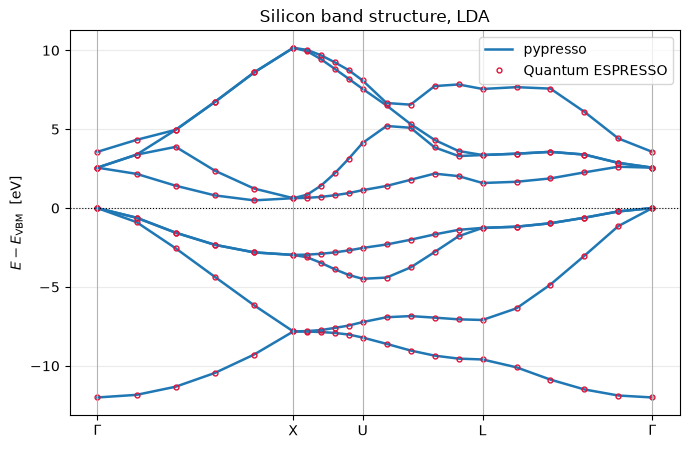
\includegraphics[width=\textwidth]{figs/02_silicon_scf_and_bands.png}
\\[2pt]
\footnotesize Silicon bands against the committed \qe\ benchmark.
\end{columns}
\end{frame}

% ---------------------------------------------------------------- 5
\begin{frame}{Densities of states, projected and total}
\begin{columns}[c]
\column{0.5\textwidth}
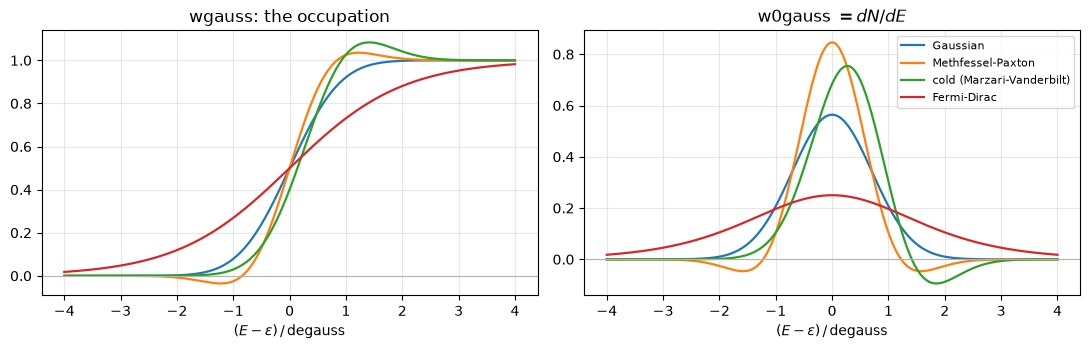
\includegraphics[width=\textwidth]{figs/06_density_of_states.png}
\column{0.5\textwidth}
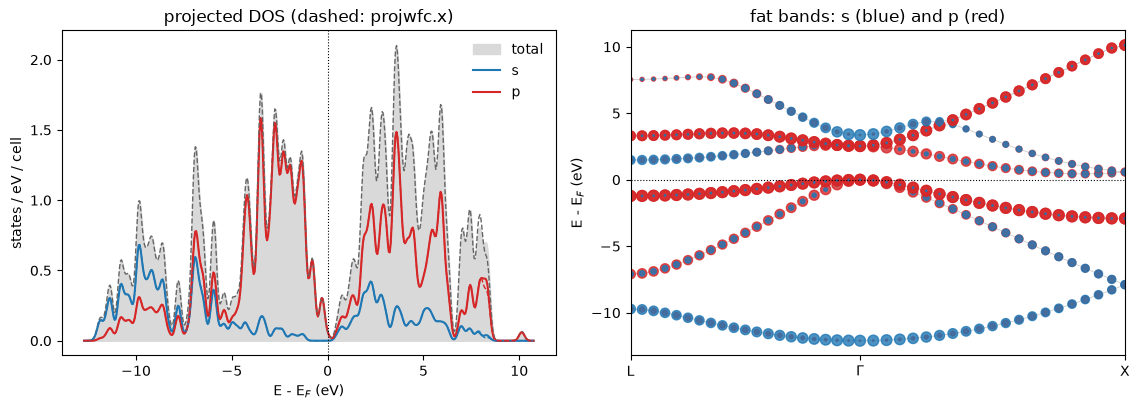
\includegraphics[width=\textwidth]{figs/16_projected_density_of_states.png}
\end{columns}
\vspace{2pt}
\footnotesize Both smearing and tetrahedron families, the latter also as an
occupation scheme inside the SCF. \textbf{PDOS} is $\langle\phi|S|\psi\rangle$ on
Löwdin-orthogonalised orbitals, matching \texttt{projwfc.x} to 6.9e-4 on a
projection and 4.7e-5 on a Löwdin charge; the spilling parameter reproduces all
four printed decimals.
\end{frame}

% ---------------------------------------------------------------- 6
\begin{frame}{Magnetism: collinear, noncollinear, spin-orbit}
\begin{columns}[c]
\column{0.5\textwidth}
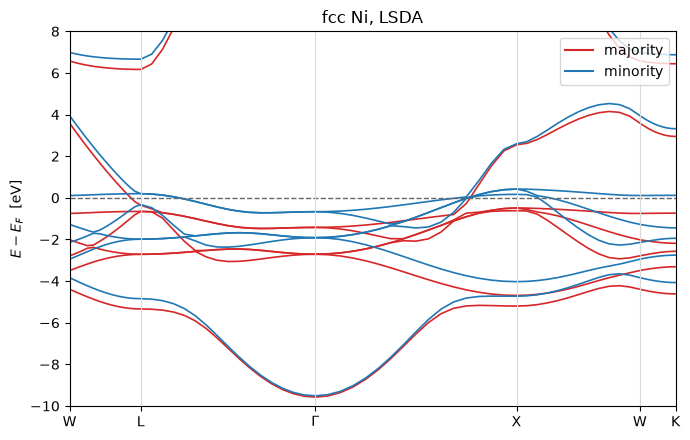
\includegraphics[width=\textwidth]{figs/07_spin_polarization.png}
\column{0.5\textwidth}
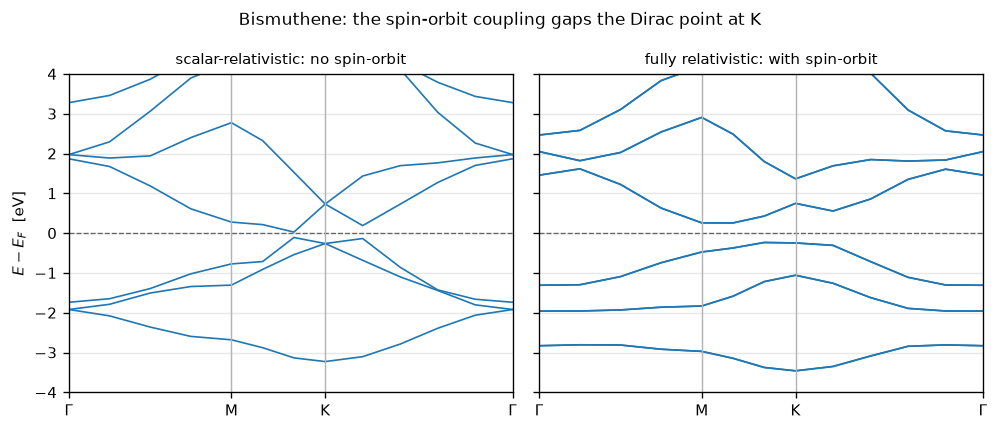
\includegraphics[width=\textwidth]{figs/08_spin_orbit_coupling.png}
\end{columns}
\vspace{2pt}
\footnotesize
\textbf{Three spin numbers are kept apart} --- \texttt{nspin} (regime),
\texttt{npol} (spinor components of a \emph{wavefunction}), \texttt{nspin\_mag}
(components of a \emph{density}) --- which is what stops a nonmagnetic
spin-orbit run allocating a magnetization it does not have. Nickel's moment:
0.7280 against the 0.73 \qe\ prints.
\end{frame}

% ---------------------------------------------------------------- 7
\begin{frame}{Forces, stress and relaxation --- one gradient, not six terms}
\begin{columns}[c]
\column{0.5\textwidth}
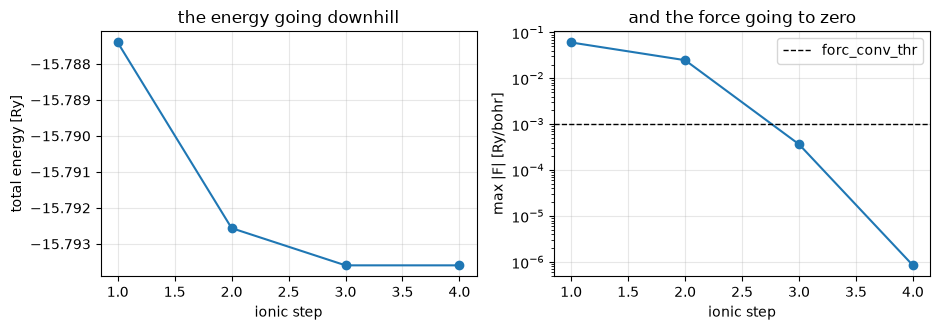
\includegraphics[width=\textwidth]{figs/09_forces_and_relaxation.png}
\column{0.5\textwidth}
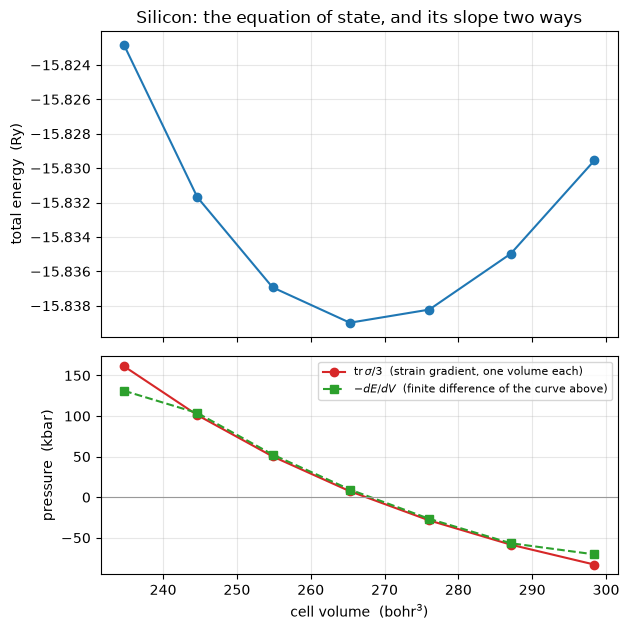
\includegraphics[width=\textwidth]{figs/15_stress.png}
\end{columns}
\vspace{2pt}
\footnotesize
The force is \texttt{jax.grad} of the total energy at frozen wavefunctions:
Hellmann-Feynman, Pulay \emph{and} the augmentation charge's own derivative all
fall out of one gradient. QE's six hand-derived terms are implemented beside it
\textbf{as a cross-check} --- which is what found the augmentation force's sign
and a missing gradient correction. Relaxed geometries reproduce \qe\ to 1e-6 bohr.
\end{frame}

% ---------------------------------------------------------------- 8
\begin{frame}{Response: dielectric, phonons, Raman}
\begin{columns}[c]
\column{0.33\textwidth}
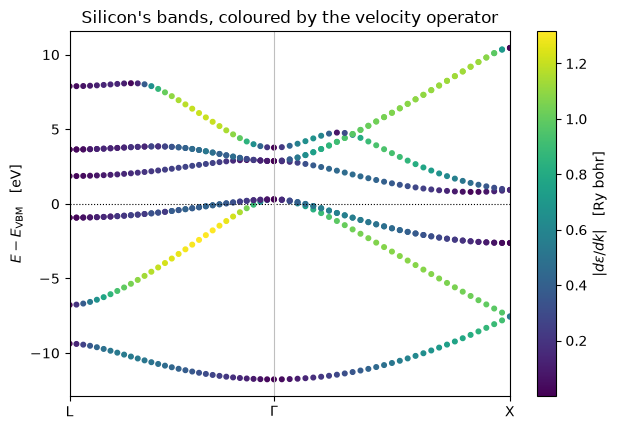
\includegraphics[width=\textwidth]{figs/19_linear_response.png}
\column{0.33\textwidth}
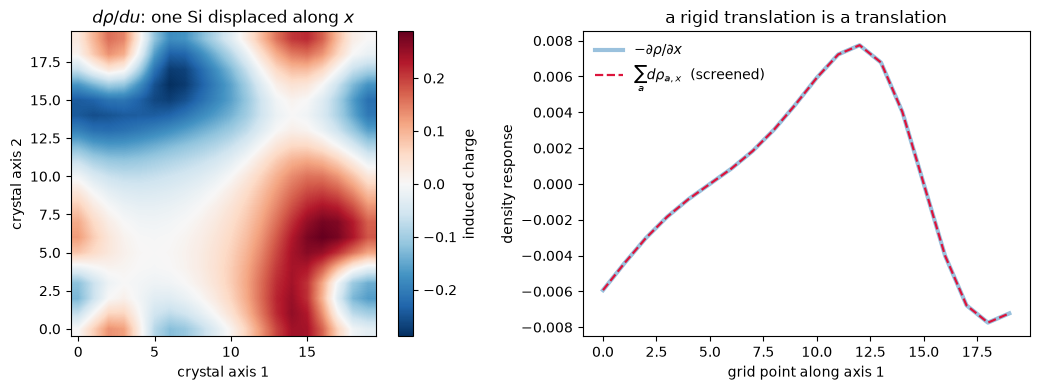
\includegraphics[width=\textwidth]{figs/20_phonons.png}
\column{0.33\textwidth}
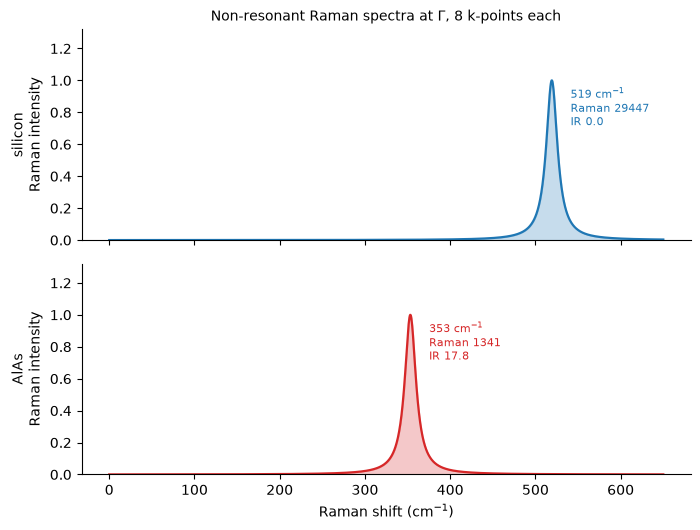
\includegraphics[width=\textwidth]{figs/26_raman_and_infrared_spectra.png}
\end{columns}
\vspace{3pt}
\footnotesize
\textbf{Sternheimer, not a sum over states} --- no empty bands, no division by
$\epsilon_n-\epsilon_m$. Silicon's $\epsilon_\infty$ matches \texttt{ph.x} to
$\le$1.2e-4 on NC, ultrasoft \emph{and} PAW; its optical mode is
\textbf{510.10\,cm$^{-1}$} against 510.15; aluminium's metal phonons agree to
\textbf{0.002\,cm$^{-1}$}. Silicon's $T_{2g}$ Raman line: \textbf{519.2\,cm$^{-1}$}
against an experimental 520 --- Raman-active and infrared-silent, which is a
symmetry statement rather than a fit.
\end{frame}

% ---------------------------------------------------------------- 9
\begin{frame}{Band gaps: the Tran-Blaha meta-GGA}
\begin{columns}[T]
\column{0.54\textwidth}
\small
\textbf{A functional whose \emph{potential} is written down and whose energy does
not exist.} \texttt{input\_dft = 'tb09'} gives the modified Becke-Johnson
meta-GGA, which fixes the gap without the cost of a hybrid.
\vspace{4pt}
\begin{tabular}{lrrr}
\toprule
 & LDA & TB09 & experiment \\
\midrule
silicon & 0.49 & \textbf{1.13} & 1.17 \\
diamond & 3.89 & \textbf{4.43} & 5.5 \\
\bottomrule
\end{tabular}
\vspace{5pt}

Validated against \emph{analytic} limits rather than another code's floating
point: the hydrogen atom, where Becke-Roussel is the exact Slater potential of
the 1s orbital to 1e-6 and $E_x$ is exactly $-5/16$\,Ha, and the uniform gas,
where the model reproduces $v_x^{\rm LDA}$ to 6e-4.
\vspace{4pt}

\footnotesize \textbf{PAW is what makes it work}: its one-centre $\tau$ comes
from the partial waves and recovers $c=1.107$ against an all-electron 1.12,
where a norm-conserving silicon measures 1.000 --- the pseudised core is exactly
what the cell average of $|\nabla\rho|/\rho$ misses.
\column{0.43\textwidth}
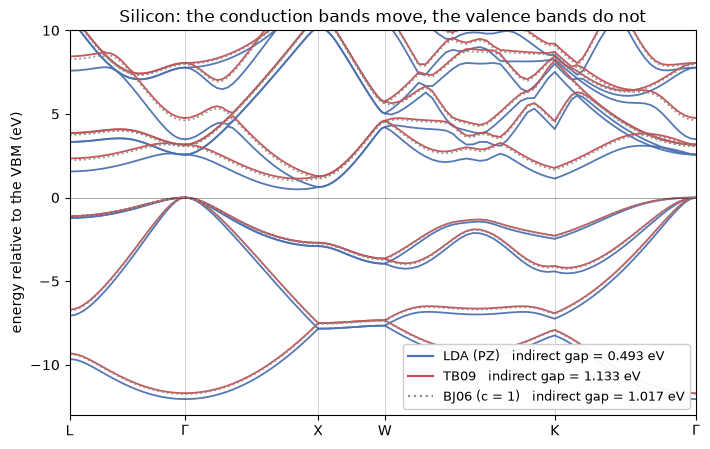
\includegraphics[width=\textwidth]{figs/24_tran_blaha_band_gaps.png}
\\[3pt]
\footnotesize
The consequences are enforced rather than documented: the total energy is
\textbf{not variational}, so forces, stress, phonons and response are
\textbf{refused by name} for this functional.
\end{columns}
\end{frame}

% ---------------------------------------------------------------- 10
\begin{frame}{GPU: nothing was ported --- what was missing was evidence}
\begin{center}
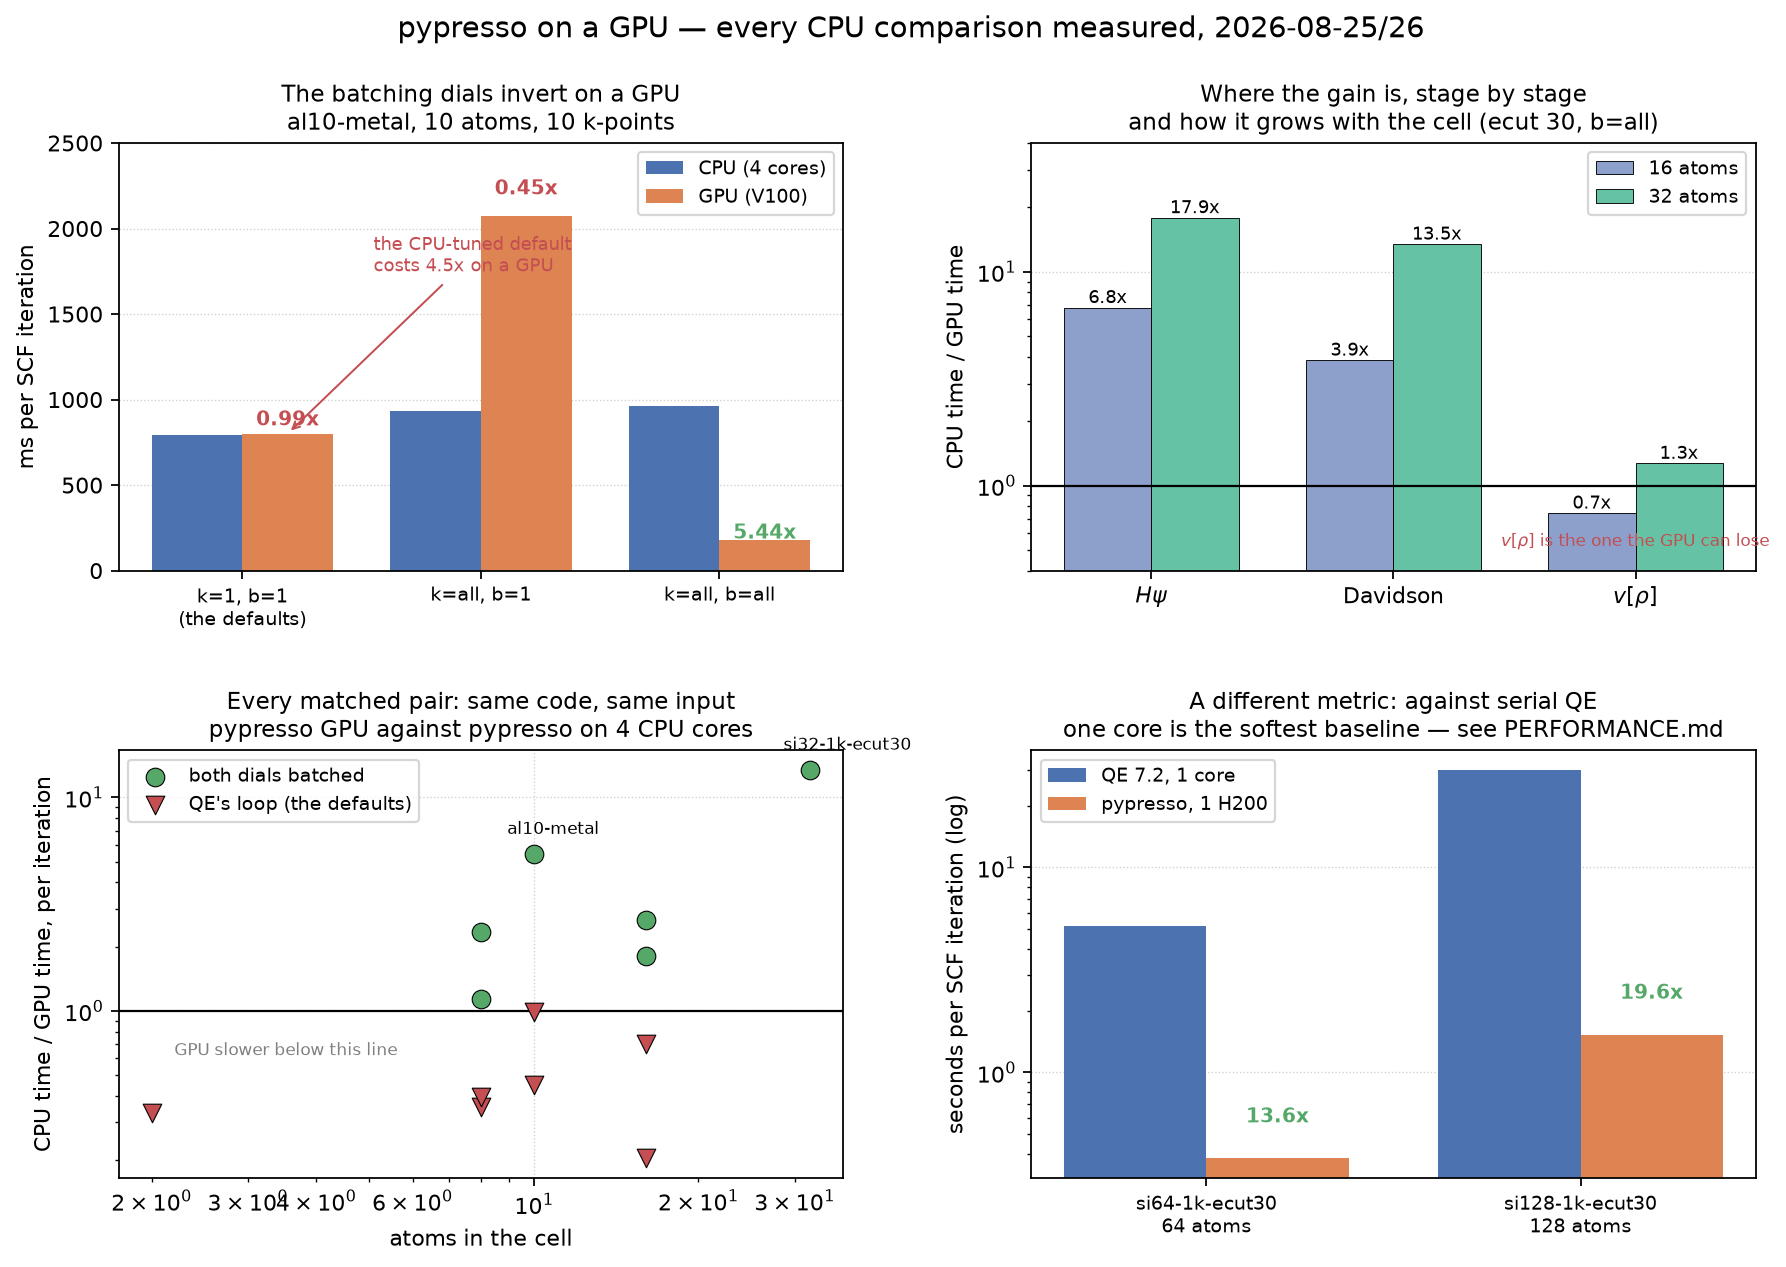
\includegraphics[width=0.93\textwidth]{figs/gpu-vs-cpu-fig.png}
\end{center}
\vspace{-4pt}
\footnotesize
JAX already emitted GPU code from this source; the rules that made that true have
bound since day one. \textbf{The finding is that the two batching dials invert}:
tuned for a CPU cache they cost \textbf{4.5x} on a GPU, and the plausible
half-measure (\texttt{k=all, b=1}) is the \emph{worst} setting available.
\end{frame}

% ---------------------------------------------------------------- 11
\begin{frame}{GPU across the physics --- 12 cases, 10--40 atoms}
\begin{center}
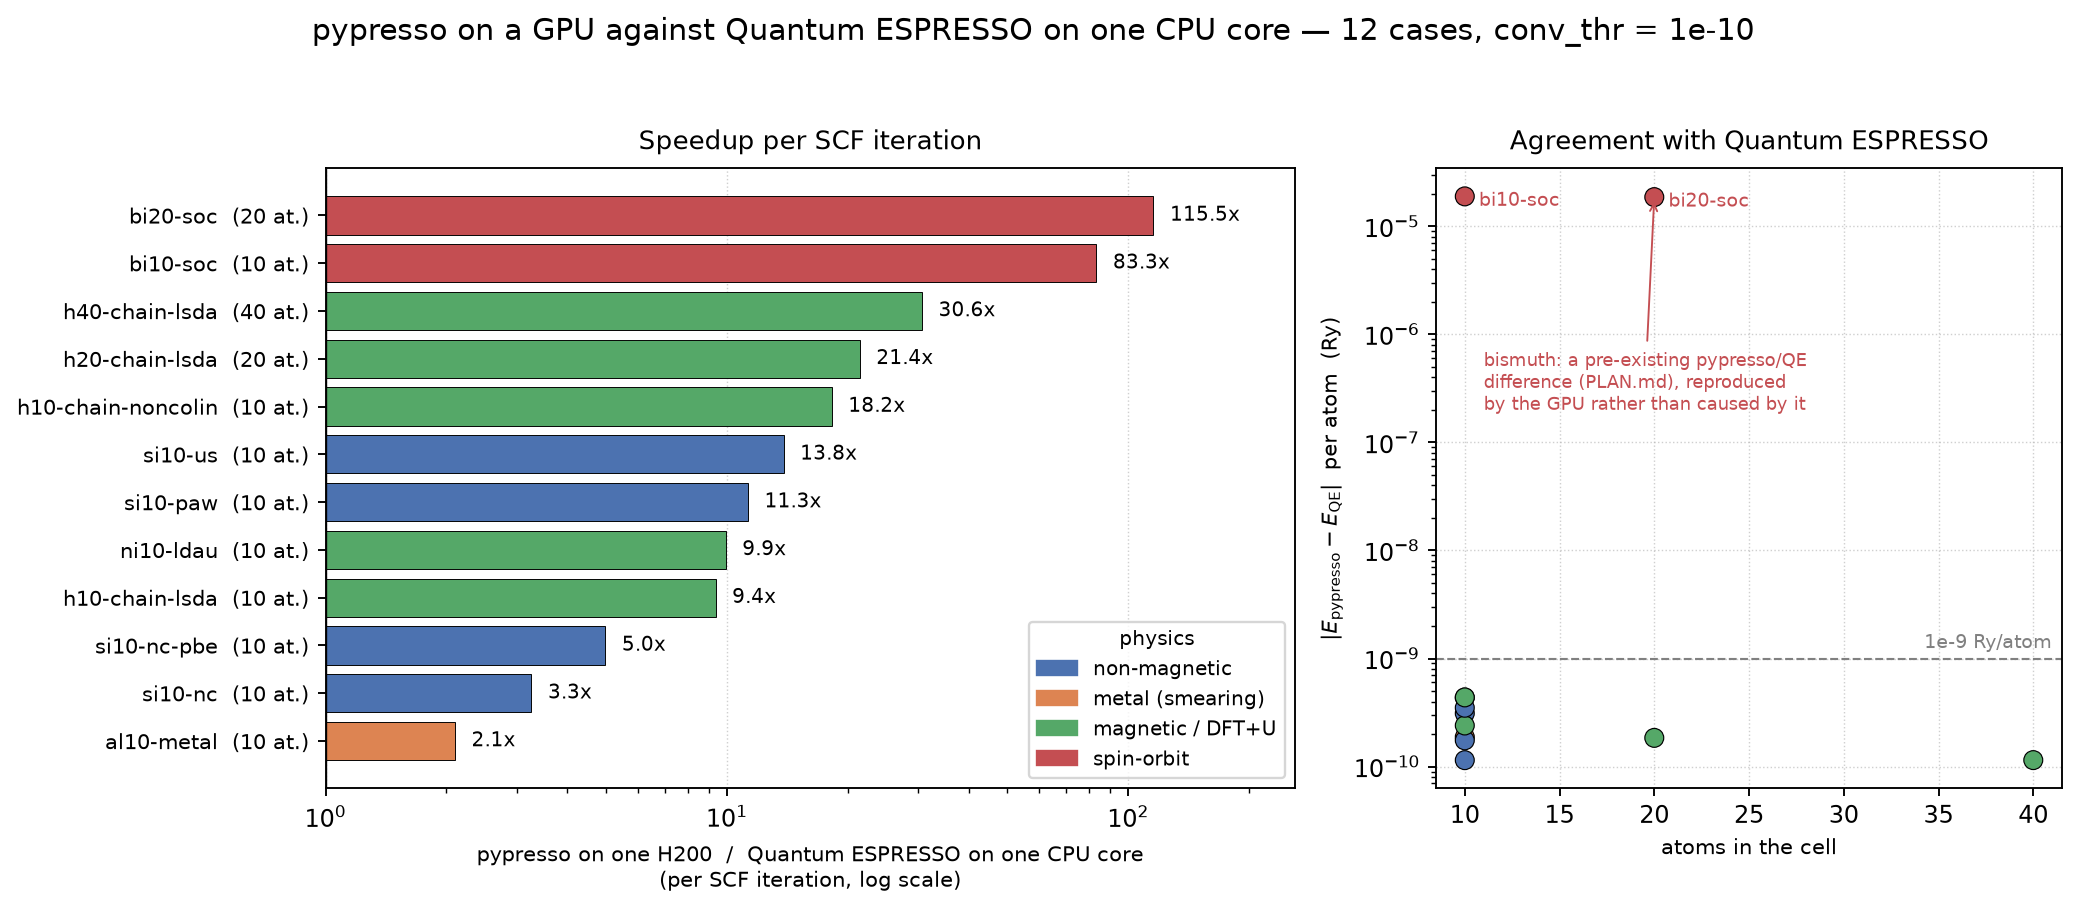
\includegraphics[width=0.95\textwidth]{figs/gpu-sweep-fig.png}
\end{center}
\vspace{-4pt}
\footnotesize
Speedup tracks \textbf{work per k-point}: 2x on a cheap metal, 9--21x with an
augmentation charge or a magnetization, \textbf{83--115x on spin-orbit}, where
serial \qe\ spends 22--105 \emph{seconds} per iteration on two-component spinors.
Energies agree to \textbf{$\sim$1e-9\,Ry} --- reproducing the \emph{CPU}
agreements already on record, including the one known bismuth discrepancy.
\end{frame}

% ---------------------------------------------------------------- 12
\begin{frame}{Where it stands}
\small
\begin{columns}[T]
\column{0.48\textwidth}
\textbf{Done}
\begin{itemize}\itemsep2pt
  \item SCF $\rightarrow$ bands $\rightarrow$ DOS, with US/PAW, GGA, all spin regimes
  \item forces, stress, relaxation, variable cell
  \item linear response, phonons, Raman/IR, electrostriction
  \item topological invariants, spin spirals (no \qe\ counterpart)
  \item \textbf{first contact with a GPU}, validated across the physics
\end{itemize}
\column{0.48\textwidth}
\textbf{Next}
\begin{itemize}\itemsep2pt
  \item phonons at $q\neq0$; $q2r$/\texttt{matdyn} dispersions
  \item $\chi^{(2)}$ and the electro-optic tensor
  \item ultrasoft dynamical matrix, PAW Born charges
  \item GPU: k-axis sharding, multi-GPU, the subspace algebra
\end{itemize}
\end{columns}
\vspace{6pt}
\hrule
\vspace{5pt}
\footnotesize
\textbf{Two habits do the work.} Every quantity is written down \emph{once} and
differentiated thereafter, with QE's hand-derived expressions kept as tests ---
so the two implementations share no machinery and disagreeing is informative.
And anything not implemented is \textbf{refused by name} rather than silently
approximated.
\end{frame}

\end{document}
